\documentclass[a4paper, 11pt]{article}
\usepackage{fullpage} % changes the margin
\usepackage{changepage}
\usepackage{amssymb,mathtools}
\usepackage{enumerate}
\usepackage{graphicx}
\usepackage{float}

\setlength{\parindent}{0pt}

\begin{document}

\large\textbf{Seven-Die Data Challenge } \hfill \textbf{Elliott Shugerman} \\


\section{Introduction}This problem is a variation on a programming challenge which I was once presented with as part of a hiring process. It has been adapted with the permission of the source. So that they may continue to administer this challenge problem, the source organization is not named, and key words have been changed in the problem statement.
 
\section{Problem}
Suppose you have a 7-sided die with sides 2, 4, 8, 16, 32, 64, and W. You decide to play the following game: roll the die repeatedly until the sum of the results exceeds a threshold $T$. Count W as 11 unless it will put you over the threshold, in which case count W as 1. Your score is the sum minus the threshold.


\begin{enumerate}[\hspace{5mm}I.]
	\item What is the mean and standard deviation of the distribution of possible scores if the threshold is 100? Give an exact answer and verify by simulation.
	\item What is the mean and standard deviation of the distribution of possible scores if the threshold is 1000? Give an exact answer and verify by simulation.
	\item What is the exact mean and standard deviation of the number of times you expect to roll the die to win the game if the threshold is 100? Give an exact answer and verify by simulation.
	\item Let the high value of W be any number. Create a visualization showing how the expected final score varies with the threshold and with the high value of W.

\end{enumerate}
 
\section{Solution}
This problem may not be solved by a brute-force approach, as the number of paths blows up quickly.

\medskip

In order to determine the distribution of scores, we will first generate the following data for each possible score: the number of roll sequences which produce the score $p$ (``paths"), and the number of rolls in each sequence $l$ (``length"). That is, we want $p_n(s)$ for $T < n < T + 64$. 

\medskip

In order to generate this function for $n > T$, we first, we first want this same function for all $n < T$. (I suppose we don't really need this data for $n < T - 64$ , but we'll find it along the way.) The rules which determine the paths to $n$ for $n < T$ depend on whether or not $n$ is greater than the ``critical point'' $n_c$.

\[ n_c = T - W_{high} + 1 \]

\pagebreak

The critical point is the number at which, when reached in a path, the value of W switches to 1. Equivalently, it is the highest number which may not be reached by a path that includes 1.\\

In summary, there are three regions, each with their own rules for choosing paths:

\medskip

\begin{adjustwidth}{3.0em}{3.0em}

	$a = (0, n_c]$ \\

	$b = (n_c, T]$ \\

	$c = (T, T + 64]$ \\

\end{adjustwidth}
\medskip

For each region, an algorithm is defined to find $p_n(l)$ for all $n$ in the region. The results for region $a$ are used to compute the results for $b$, the results for $a$ and $b$ are used to compute the results for $c$. These algorithms are described in the section below.\\

From here, we are nearly ready to calculate our final results. But one step of legwork remains -- we must take into account that the probability a particular path will be traversed is not equal for all paths. When a single path branches into two, the relative probability that either child branch will be traversed is $1/2$ to the parent's 1; a second branching will create paths with probability $1/2^2$. In our case, 7 branches diverge each step of the way, so the relative probability that a path with $l$ steps will be traversed is $1/l^2$. Thus, we must scale our $p_n(l)$ distributions for each score in the following manner:

\[ p_n^t(l) = (1 / l^2)p_n(l) \]

where $p_n^t$ is the (un-normalized) distribution of paths \textit{actually taken} and $p_n$ is the distribution of paths which \textit{exist} or \textit{could be taken}.\\

Finally, we can now construct our score distribution. The relative probability for each score is the sum of the corresponding $p_n^t(l)$ over $l$.

\subsection{Counting Algorithms}


NOTE 1: The algorithms below merely count the number of paths to a number n. However, the number of paths \textit{for each path length} is needed to solve the problem. The functions in the python code are essentially equivalent to those here, except instead of returning a single number, they return a distribution as a dict, with path length $l$ as keys and multiplicity as values. These functions call each other (or lookup data computed by the others). When the dict P(n) is computed as a sum, and P(m) is an element in this sum, the value $P(m)|(l=l_0)$ is added to (the accumulator for) $P(n)|l = l_0 + 1$.\\ 


NOTE 2: The algorithms for regions $a$ and $b$ are actually implemented in the same python function, \texttt{count\_paths}, but are described here as seperate for clarity. The algorithm for region $c$ is implemented in \texttt{count\_paths\_end}.\\


\pagebreak

DEFINITIONS:

\begin{adjustwidth}{3.0em}{3.0em}
$P_r(n)$ is the number of paths to $n$ where $n \in r$\\

$L = \{1, 2, 4, . . . , 64\}$ \\

$H = \{11, 2, 4, . . . , 64\}$ \\

\end{adjustwidth}

\subsubsection{region a}
domain: $n \vert n < n_c$

\[
	P_a(n) = \sum_{i=0}^{\vert H \vert}
		\begin{cases}
			P_a(n - H_i)	& \text{if $n - H_i > 0$} \\
			1		& \text{if $n - H_i = 0$} \\
			0		& \text{if $n - H_i < 0$}
		 \end{cases}
\]

\subsubsection{region b}
domain: $n \vert n < T$

\[
	P_b(n) = \sum_{i=0}^{\vert L \vert}
		\begin{cases}
			P_a(n - L_i)	& \text{if $n - L_i \leq n_c$} \\
			P_b(n - L_i)	& \text{otherwise} \\
		 \end{cases}
\]

\subsubsection{region c}
domain: $n \vert T < n < T + 64$
\[
	P_c(n) = \sum_{i=0}^{\vert L \vert}
		\begin{cases}
			P_b(n - L_i)	& \text{if $n - L_i \leq T$} \\
			0		& \text{otherwise}
			
		 \end{cases}
\]



\begin{figure}[H]
  \centering
  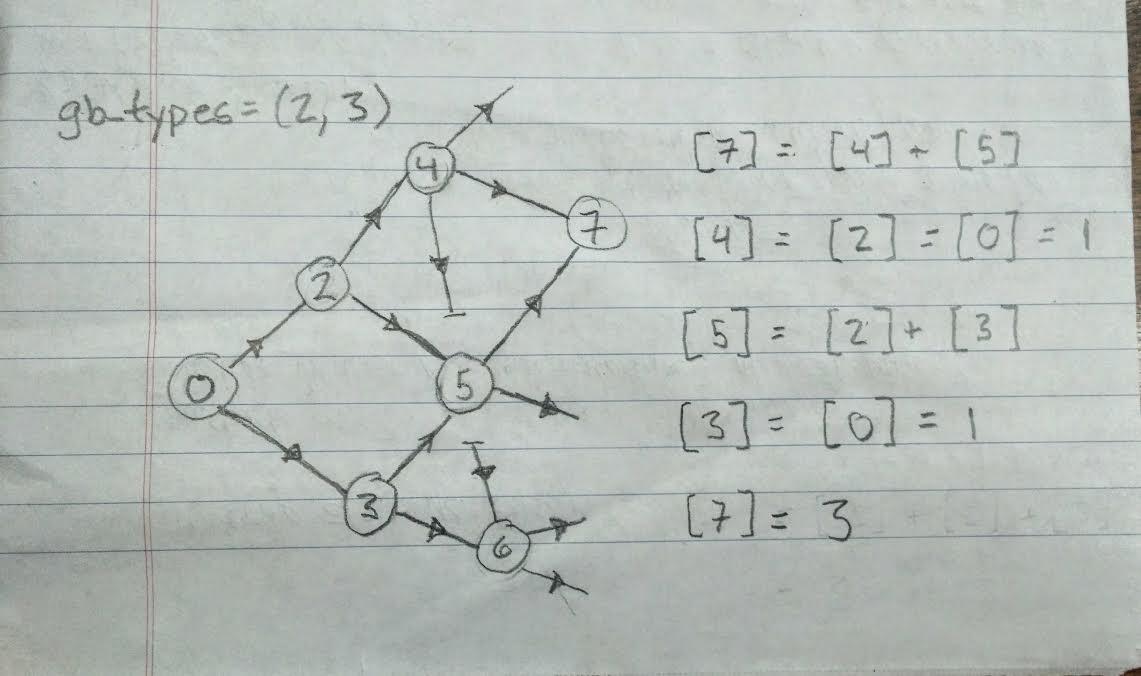
\includegraphics[scale=.3]{diagram.jpg}
  \caption{Possible games paths as a DAG, motivating the algorithms above. Here, [n] denotes the number of paths to a sum n, and the die is a two-sided die (a coin?) yielding either 2 or 3.}
\end{figure}


\end{document}

